\section{C}
To prove that \textsc{MirrorFriendlyMinimumSpanningTree}, (\textsc{Mfmst}), is $\mathcal{NP}$-complete we need to choose a suitable problem $P_c$. \textsc{PartitionByPairs} is already known to be $\mathcal{NP}$-complete and so for this proof $P_c = \textsc{PartitionByPairs}$.

Now we want to prove that
\begin{align*}
    P_c &\leq_p \textsc{Mfmst} \Rightarrow \\
    \textsc{PartitionByPairs} &\leq_p \textsc{Mfmst}
\end{align*}

\subsection{Transformation}
We will do this by describing a transformation of \textsc{PartitionByPairs} into \textsc{Mfmst}. The input for the transformation is an instance of \textsc{PartitionByPairs}, that is a sequence of natural numbers $S = \left(s_1,s_2,\ldots,s_{2n} \right)$.

In \textsc{PartitionByPairs} the numbers in $S$ are split into pairs, we will use these pairs to construct a graph for \textsc{Mfmst}. 

The graph is constructed in two steps. The first half if the graph consists of $n+1$ vertices
\begin{align*}
    V_1 = (v_1,v_2,v_3,\ldots,v_{n-1},v_n,v_n+1)
\end{align*}
where there is an edge between the neighbours in $V_1$. This is illustrated below.

\noindent\begin{minipage}{\textwidth}
	\centering
	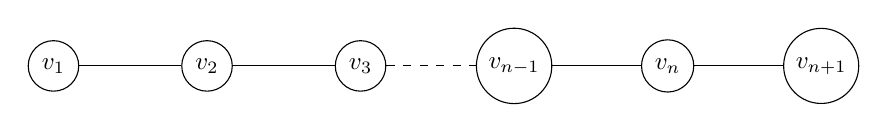
\begin{tikzpicture}
        [scale=0.65,auto=left,every node/.style={circle,draw,scale=.9}]
        %Left side
        \node  (V1) at (0,0)			    {$v_1$};
		\node  (V2) at (3,0)			    {$v_2$};
		\node  (V3) at (6,0)                {$v_3$};
		\node  (VN-1) at (9,0)              {$v_{n-1}$};
		\node  (VN) at (12,0)               {$v_n$};
		\node  (VN+1) at (15,0)			    {$v_{n+1}$};
        
        \draw[pos=0.17, above=10pt, every node/.style={sloped,anchor=south,auto=false}]
  		(V1)	    edge		node {}	(V2)
  		(V2)	    edge		node {}	(V3)
  		(VN-1)      edge        node {} (VN)
  		(VN)	    edge		node {}	(VN+1);
  		
  		\draw[dashed, pos=0.17, above=10pt, every node/.style={sloped,anchor=south,auto=false}]
  		(V3)	    edge		node {}	(VN-1);
    \end{tikzpicture}
\end{minipage}
\\

The sequence of edges between the vertices in $V_1$ is called 
\begin{align*}
    E_1 = (\{v_1, v_2\}, \{v_2,v_3\},\ldots \{v_{n-1},v_n\}, \{v_n,v_{n+1}\})   
\end{align*}
The first number of each pair $S_1 = (s_1,s_3,\ldots,s_{2n-3},s_{2n-1})$, are used as weights for the edges in the first half of the graph. The first number in $S_1$ is used as weight for the first edge, the edge between $v_1$ and $v_2$, in the first half of the graph, as shown below

\noindent\begin{minipage}{\textwidth}
	\centering
	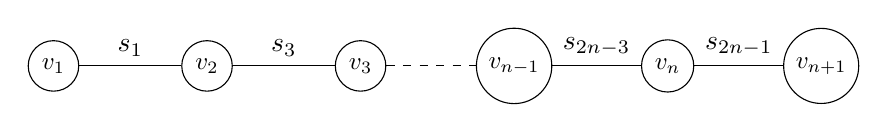
\begin{tikzpicture}
        [scale=0.65,auto=left,every node/.style={circle,draw,scale=.9}]
        %Left side
        \node  (V1) at (0,0)			    {$v_1$};
		\node  (V2) at (3,0)			    {$v_2$};
		\node  (V3) at (6,0)                {$v_3$};
		\node  (VN-1) at (9,0)              {$v_{n-1}$};
		\node  (VN) at (12,0)               {$v_n$};
		\node  (VN+1) at (15,0)			    {$v_{n+1}$};
        
        \draw[above=10pt, every node/.style={sloped,anchor=south,auto=false}]
  		(V1)	    edge		node {$s_1$}	(V2)
  		(V2)	    edge		node {$s_3$}	(V3)
  		(VN-1)      edge        node {$s_{2n-3}$} (VN)
  		(VN)	    edge		node {$s_{2n-1}$}	(VN+1);
  		
  		\draw[dashed, above=10pt, every node/.style={sloped,anchor=south,auto=false}]
  		(V3)	    edge		node {}	(VN-1);
    \end{tikzpicture}
\end{minipage}
\\

The second half of the graph consists of $n+1$ vertices,
\begin{align*}
    U_1 = (u_1,u_2,u_3,\ldots,u_{n-1},u_n,u_{n+1})
\end{align*}
and there are edges between the vertices in $U_1$ as there is in $V_1$. The sequence of edges between the vertices in $U_1$ is called
\begin{align*}
    E_2 = (\{u_n,u_{n+1}\}, \{u_{n-1},u_n\}, \ldots, \{v_2,v_3\}, \{v_1, v_2\})
\end{align*}
Notice that the order of the edges in $E_2$ is reversed compared to the order in $E_1$. The weights for the edges between the vertices in $U_1$ is made up of the second numbers in the pairs, so the sequence $S_2 = (s_2,s_4,\ldots,s_{2n-2},s_{2n})$. Finally to connect the two halves of the graph, an edge between the corresponding vertices in $V_1$ and $U_1$ with a weight of 0 is inserted, that is a total of $n+1$ edges with a weight of 0. The sequence of edges with 0 weight will called $E_3$. The complete graph looks as follows

\noindent\begin{minipage}{\textwidth}
	\centering
	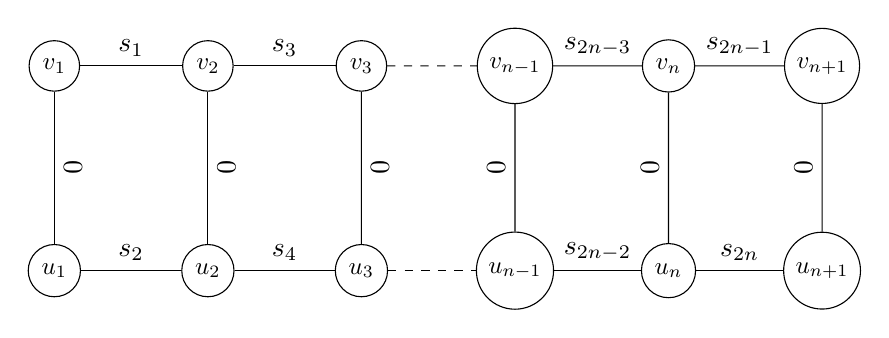
\begin{tikzpicture}
        [scale=0.65,auto=left,every node/.style={circle,draw,scale=.9}]
        % V_1
        \node  (V1) at      (0,4)			{$v_1$};
		\node  (V2) at      (3,4)		    {$v_2$};
		\node  (V3) at      (6,4)           {$v_3$};
		\node  (VN-1) at    (9,4)           {$v_{n-1}$};
		\node  (VN) at      (12,4)          {$v_n$};
		\node  (VN+1) at    (15,4)			{$v_{n+1}$};
		
		% U_1
		\node  (U1) at (0,0)			    {$u_1$};
		\node  (U2) at (3,0)			    {$u_2$};
		\node  (U3) at (6,0)                {$u_3$};
		\node  (UN-1) at (9,0)              {$u_{n-1}$};
		\node  (UN) at (12,0)               {$u_n$};
		\node  (UN+1) at (15,0)			    {$u_{n+1}$};
        
        \draw[above=10pt, every node/.style={sloped,anchor=south,auto=false}]
  		(V1)	    edge		node {$s_1$}        (V2)
  		(V2)	    edge		node {$s_3$}	    (V3)
  		(VN-1)      edge        node {$s_{2n-3}$}   (VN)
  		(VN)	    edge		node {$s_{2n-1}$}	(VN+1)
  		
  		(U1)	    edge		node {$s_2$}	    (U2)
  		(U2)	    edge		node {$s_4$}	    (U3)
  		(UN-1)      edge        node {$s_{2n-2}$}   (UN)
  		(UN)	    edge		node {$s_{2n}$}	    (UN+1)
  		
  		% 0 edges.
  		(V1)	    edge		node {0}            (U1)
  		(V2)	    edge		node {0}            (U2)
  		(V3)	    edge		node {0}            (U3)
  		(VN-1)	    edge		node {0}            (UN-1)
  		(VN)	    edge		node {0}            (UN)
  		(VN+1)	    edge		node {0}            (UN+1);
  		
  		\draw[dashed, above=10pt, every node/.style={sloped,anchor=south,auto=false}]
  		(V3)	    edge		node {}	(VN-1)
  		(U3)	    edge		node {}	(UN-1);
    \end{tikzpicture}
\end{minipage}
\\

The complete sequence of edges looks as follows 
\begin{align*}
    E = (E_1, E_3, E_2)
\end{align*}
This means that if $w(e_i)$ is a number from the sequence $S$, then the other number in the pair from the \textsc{PartitionByPairs} problem is $w(e_{m+1-i})$.

The complete set of vertices will be
\begin{align*}
    V = V_1 \cup U_1
\end{align*}
and $w$ gives the weight of the edges in the way that was described in this section. This gives us the graph $G=(V,E,w)$. Finally let
\begin{align*}
    B = \frac{1}{2} \sum_{x \in S} x
\end{align*}

For the transformation a graph is created with $2(n+1)$ vertices with $m = 3n+1$ edges. A graph can be created in polynomial time in the amount of vertices and edges. $B$ is calculated by the sum of the numbers in $S$, which can be done in polynomial time in the amount of numbers. In other words the transformation can be done in polynomial time.

% Proof YES to PartitionByPairs gives YES to MFMST
\subsection{PartitionByPairs $\Rightarrow$ MFMST}
Consider an assignment of the subset $A$ that choose exactly one from each pair $(2i-1,2i)$, where $i \in \{1,\ldots,n\}$, such that $\sum_{i \in A} s_i = \sum_{i \in \{1,\ldots,2n\}\setminus A} s_i$.
We will now show that there is a spanning tree $T'$ such that
\begin{align*}
    max \left\{ \sum_{e_i \in T'} w(e_i), \sum_{e_i \in T'} w(e_{m+1-i}) \right\} \leq B
\end{align*}
We will construct the spanning tree in the following way. For each $i \in A$ add the edge where $s_i$ is the weight and all the edges in $E_3$, that is all the edges with weight zero.

Example with $n = 4$ and $A = \{1,4,6,7\}$, gives the following sequence of edges
\begin{align*}
    \{s_1, s_3, s_5, s_7, 0, 0, 0, 0, 0, s_8, s_6, s_4, s_2\}
\end{align*}

\noindent\begin{minipage}{\textwidth}
	\centering
	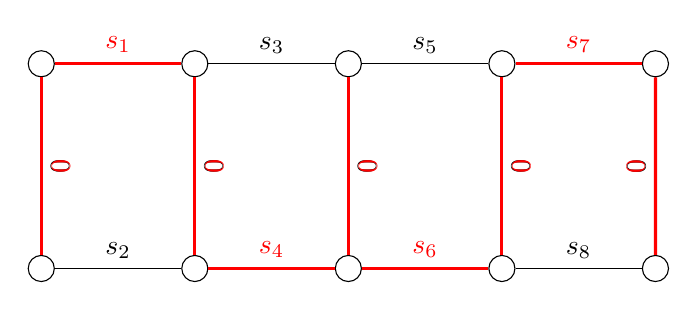
\begin{tikzpicture}
        [scale=0.65,auto=left,every node/.style={circle,draw,scale=1}]
        % V_1
        \node  (V1) at      (0,4)			{};
		\node  (V2) at      (3,4)		    {};
		\node  (V3) at      (6,4)           {};
		\node  (V4) at      (9,4)           {};
		\node  (V5) at      (12,4)          {};
		
		% U_1
		\node  (U1) at      (0,0)			{};
		\node  (U2) at      (3,0)		    {};
		\node  (U3) at      (6,0)           {};
		\node  (U4) at      (9,0)           {};
		\node  (U5) at      (12,0)          {};
        
        \draw[above=10pt, every node/.style={sloped,anchor=south,auto=false}]
  		(V2)	    edge		node {$s_3$}	    (V3)
  		(V3)        edge        node {$s_5$}        (V4)
  		(U1)	    edge		node {$s_2$}	    (U2)
  		(U4)	    edge		node {$s_8$}	    (U5)
  		
  		% 0 edges.
  		(V1)	    edge		node {0}            (U1)
  		(V2)	    edge		node {0}            (U2)
  		(V3)	    edge		node {0}            (U3)
  		(V4)	    edge		node {0}            (U4)
  		(V5)	    edge		node {0}            (U5);
  		
  		\draw[line width=0.4mm, red, above=10pt, every node/.style={sloped,anchor=south,auto=false}]
  		(V1)	    edge		node {$s_1$}        (V2)
  		(V4)	    edge		node {$s_7$}	    (V5)
  		(U2)	    edge		node {$s_4$}	    (U3)
  		(U3)        edge        node {$s_6$}        (U4)
        (V1)	    edge		node {0}            (U1)
  		(V2)	    edge		node {0}            (U2)
  		(V3)	    edge		node {0}            (U3)
  		(V4)	    edge		node {0}            (U4)
  		(V5)	    edge		node {0}            (U5);
    \end{tikzpicture}
\end{minipage}
\\

The sub-graph, marked with red, is always connected as all the 0-edges are chosen as well as one edge from each pair. The amount of chosen edges is $2 \cdot n + 1$, which is one less than the number of vertices. Therefore it must be a spanning tree as it is connected. The accumulated weight of the edges in the spanning tree corresponds to the sum $\sum_{i \in A} s_i$ in \textsc{PartitionByPairs}, as we only choose 0-edges and edges with the numbers specified by $A$. The mirror of $T'$ consists of all the edges that is not specified by $A$ as well as the 0-edges. The weight of this corresponds to the sum $\sum_{i \in \{1,\ldots,2n\}\setminus A} s_i$ in \textsc{PartitionByPairs}. 
So we have that
\begin{align*}
    \sum_{e_i \in T'} w(e_i) &= \sum_{i \in A} s_i  \\
    \sum_{e_i \in T'} w(e_{m+1-i}) &= \sum_{i \in \{1,\ldots,2n\}\setminus A} s_i
\end{align*}
It is given that
\begin{align*}
    B &= \frac{1}{2} \sum_{x \in S} x \\
    \sum_{i \in A} s_i &= \sum_{i \in \{1,\ldots,2n\}\setminus A} s_i
\end{align*}
So we have that
\begin{align*}
    2B = \sum_{i \in A} s_i &+ \sum_{i \in \{1,\ldots,2n\}\setminus A} s_i \Rightarrow \\
    2B = \sum_{e_i \in T'} w(e_i) &+ \sum_{e_i \in T'} w(e_{m+1-i})
\end{align*}
and
\begin{align*}
    \sum_{e_i \in T'} w(e_i) = \sum_{e_i \in T'} w(e_{m+1-i})
\end{align*}
Then we have that
\begin{align*}
    2B &= \sum_{e_i \in T'} w(e_i) + \sum_{e_i \in T'} w(e_{m+1-i}) \Rightarrow \\
    2B &= \sum_{e_i \in T'} w(e_i) + \sum_{e_i \in T'} w(e_i) \Rightarrow \\
    2B &= 2\sum_{e_i \in T'} w(e_i) \Rightarrow\\
    B &= \sum_{e_i \in T'} w(e_i)
\end{align*}
Likewise
\begin{align*}
    2B &= \sum_{e_i \in T'} w(e_i) + \sum_{e_i \in T'} w(e_{m+1-i}) \Rightarrow \\
    2B &= \sum_{e_i \in T'} w(e_{m+1-i}) + \sum_{e_i \in T'} w(e_{m+1-i}) \Rightarrow \\
    2B &= 2\sum_{e_i \in T'} w(e_{m+1-i}) \Rightarrow\\
    B &= \sum_{e_i \in T'} w(e_{m+1-i})
\end{align*}
Then the answer is YES to $T(X)$

\subsection{MFMST $\Rightarrow$ PartitionByPairs}
Consider a solution to \textsc{Mfmst} $T'$ then we want to show that the answer to the \textsc{PartitionByPairs} problem is YES.

We will first argue that $T'$ will contain at least one edge with a value from each pair. A cut from a graph will look like the following.

\noindent\begin{minipage}{\textwidth}
	\centering
	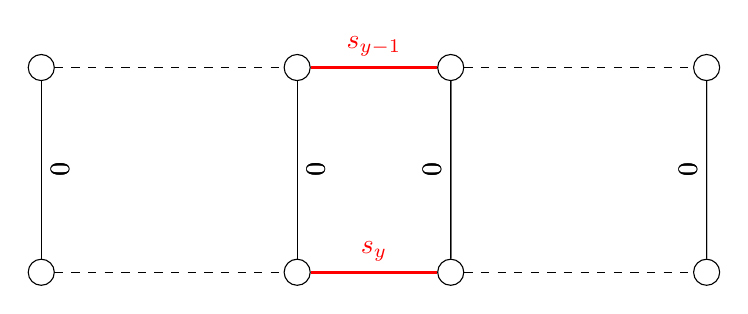
\begin{tikzpicture}
        [scale=0.65,auto=left,every node/.style={circle,draw,scale=1}]
        % V_1
        \node  (V1) at      (0,4)			{};
		\node  (V2) at      (5,4)		    {};
		\node  (V3) at      (8,4)           {};
		\node  (V4) at      (13,4)           {};
		
		% U_1
		\node  (U1) at      (0,0)			{};
		\node  (U2) at      (5,0)		    {};
		\node  (U3) at      (8,0)           {};
		\node  (U4) at      (13,0)           {};
        
        \draw[above=10pt, every node/.style={sloped,anchor=south,auto=false}]
  		(V1)	    edge		node {0}            (U1)
  		(V2)	    edge		node {0}            (U2)
  		(V3)	    edge		node {0}            (U3)
  		(V4)	    edge		node {0}            (U4)
  		
  		% 0 edges.
  		(V1)	    edge		node {0}            (U1)
  		(V2)	    edge		node {0}            (U2)
  		(V3)	    edge		node {0}            (U3)
  		(V4)	    edge		node {0}            (U4);
  		
  		\draw[line width=0.4mm, red, above=10pt, every node/.style={sloped,anchor=south,auto=false}]
  		(V2)	    edge		node {$s_{y-1}$}	(V3)
  		(U2)	    edge		node {$s_y$}	    (U3);

  		\draw[dashed, pos=0.17, above=10pt, every node/.style={sloped,anchor=south,auto=false}]
  		(V1)	    edge		node {}             (V2)
  		(V3)        edge        node {}             (V4)
  		(U1)	    edge		node {}     	    (U2)
  		(U3)        edge        node {}             (U4);
    \end{tikzpicture}
\end{minipage}
\\

Since $T'$ is a spanning tree it will contain at least one of the red edges, $s_{y-1}, s_y$. This is the case for all pairs, meaning that it will choose at least one number from each pair in \textsc{PartitionByPairs}. Knowing that, we will now show that it can not contain more than one from each pair. 

Assume that $T'$ contains both red edges for some cut in the graph, then both numbers $s_{y-1}, s_y$ will be included in both sums in
\begin{align*}
    max \left\{ \sum_{e_i \in T'} w(e_i), \sum_{e_i \in T'} w(e_{m+1-i}) \right\} \leq B
\end{align*}
Since we have to include at least one number from each pair in the spanning tree $T'$, all the numbers from $S$ will be in one of the two sums. $2B$ is the sum of all numbers in $S$. It is given that all number in $S$ are natural numbers. This means that $s_{y-1}, s_y$ appear in both sums. That gives
\begin{align*}
    \sum_{e_i \in T'} w(e_i) + \sum_{e_i \in T'} w(e_{m+1-i}) > 2B
\end{align*}
This means that at least one of the sums is greater than B. So if $T'$ contains both $s_{y-1}, s_y$, then it is not a solution, meaning that $T'$ must contain exactly one of $s_{y-1}, s_y$.

$2B$ is the sum of all numbers in $S$ and because chose one number from each pair, all number will appear in one of the sums. Furthermore nor is either of the sums greater than $B$ and the sum of both sums, which is then the sum of all numbers in $S$, is equal to $2B$. From this we can conclude that both sums are equal.

With this knowledge, we find a solution to the \textsc{PartitionByPairs} problem, where we choose $A$ to correspond to the edges in $T'$ which exists in $S$. Then we know that we have chosen exactly one number from each pair, and that 
\begin{align*}
    \sum_{i \in A} s_i &= \sum_{e_i \in T'} w(e_i) \\
    \sum_{i \in \{1,\ldots,2n\}\setminus A} s_i &= \sum_{e_i \in T'} w(e_{m+1-i}) \\
    \sum_{i \in A} s_i &= \sum_{i \in \{1,\ldots,2n\}\setminus A} s_i = B
\end{align*}
This corresponds to a solution in the \textsc{PartitionByPairs} problem.

This completes the proof. 